\begin{figure*}
\begin{subfigure}[t]{\textwidth}
    \centering
	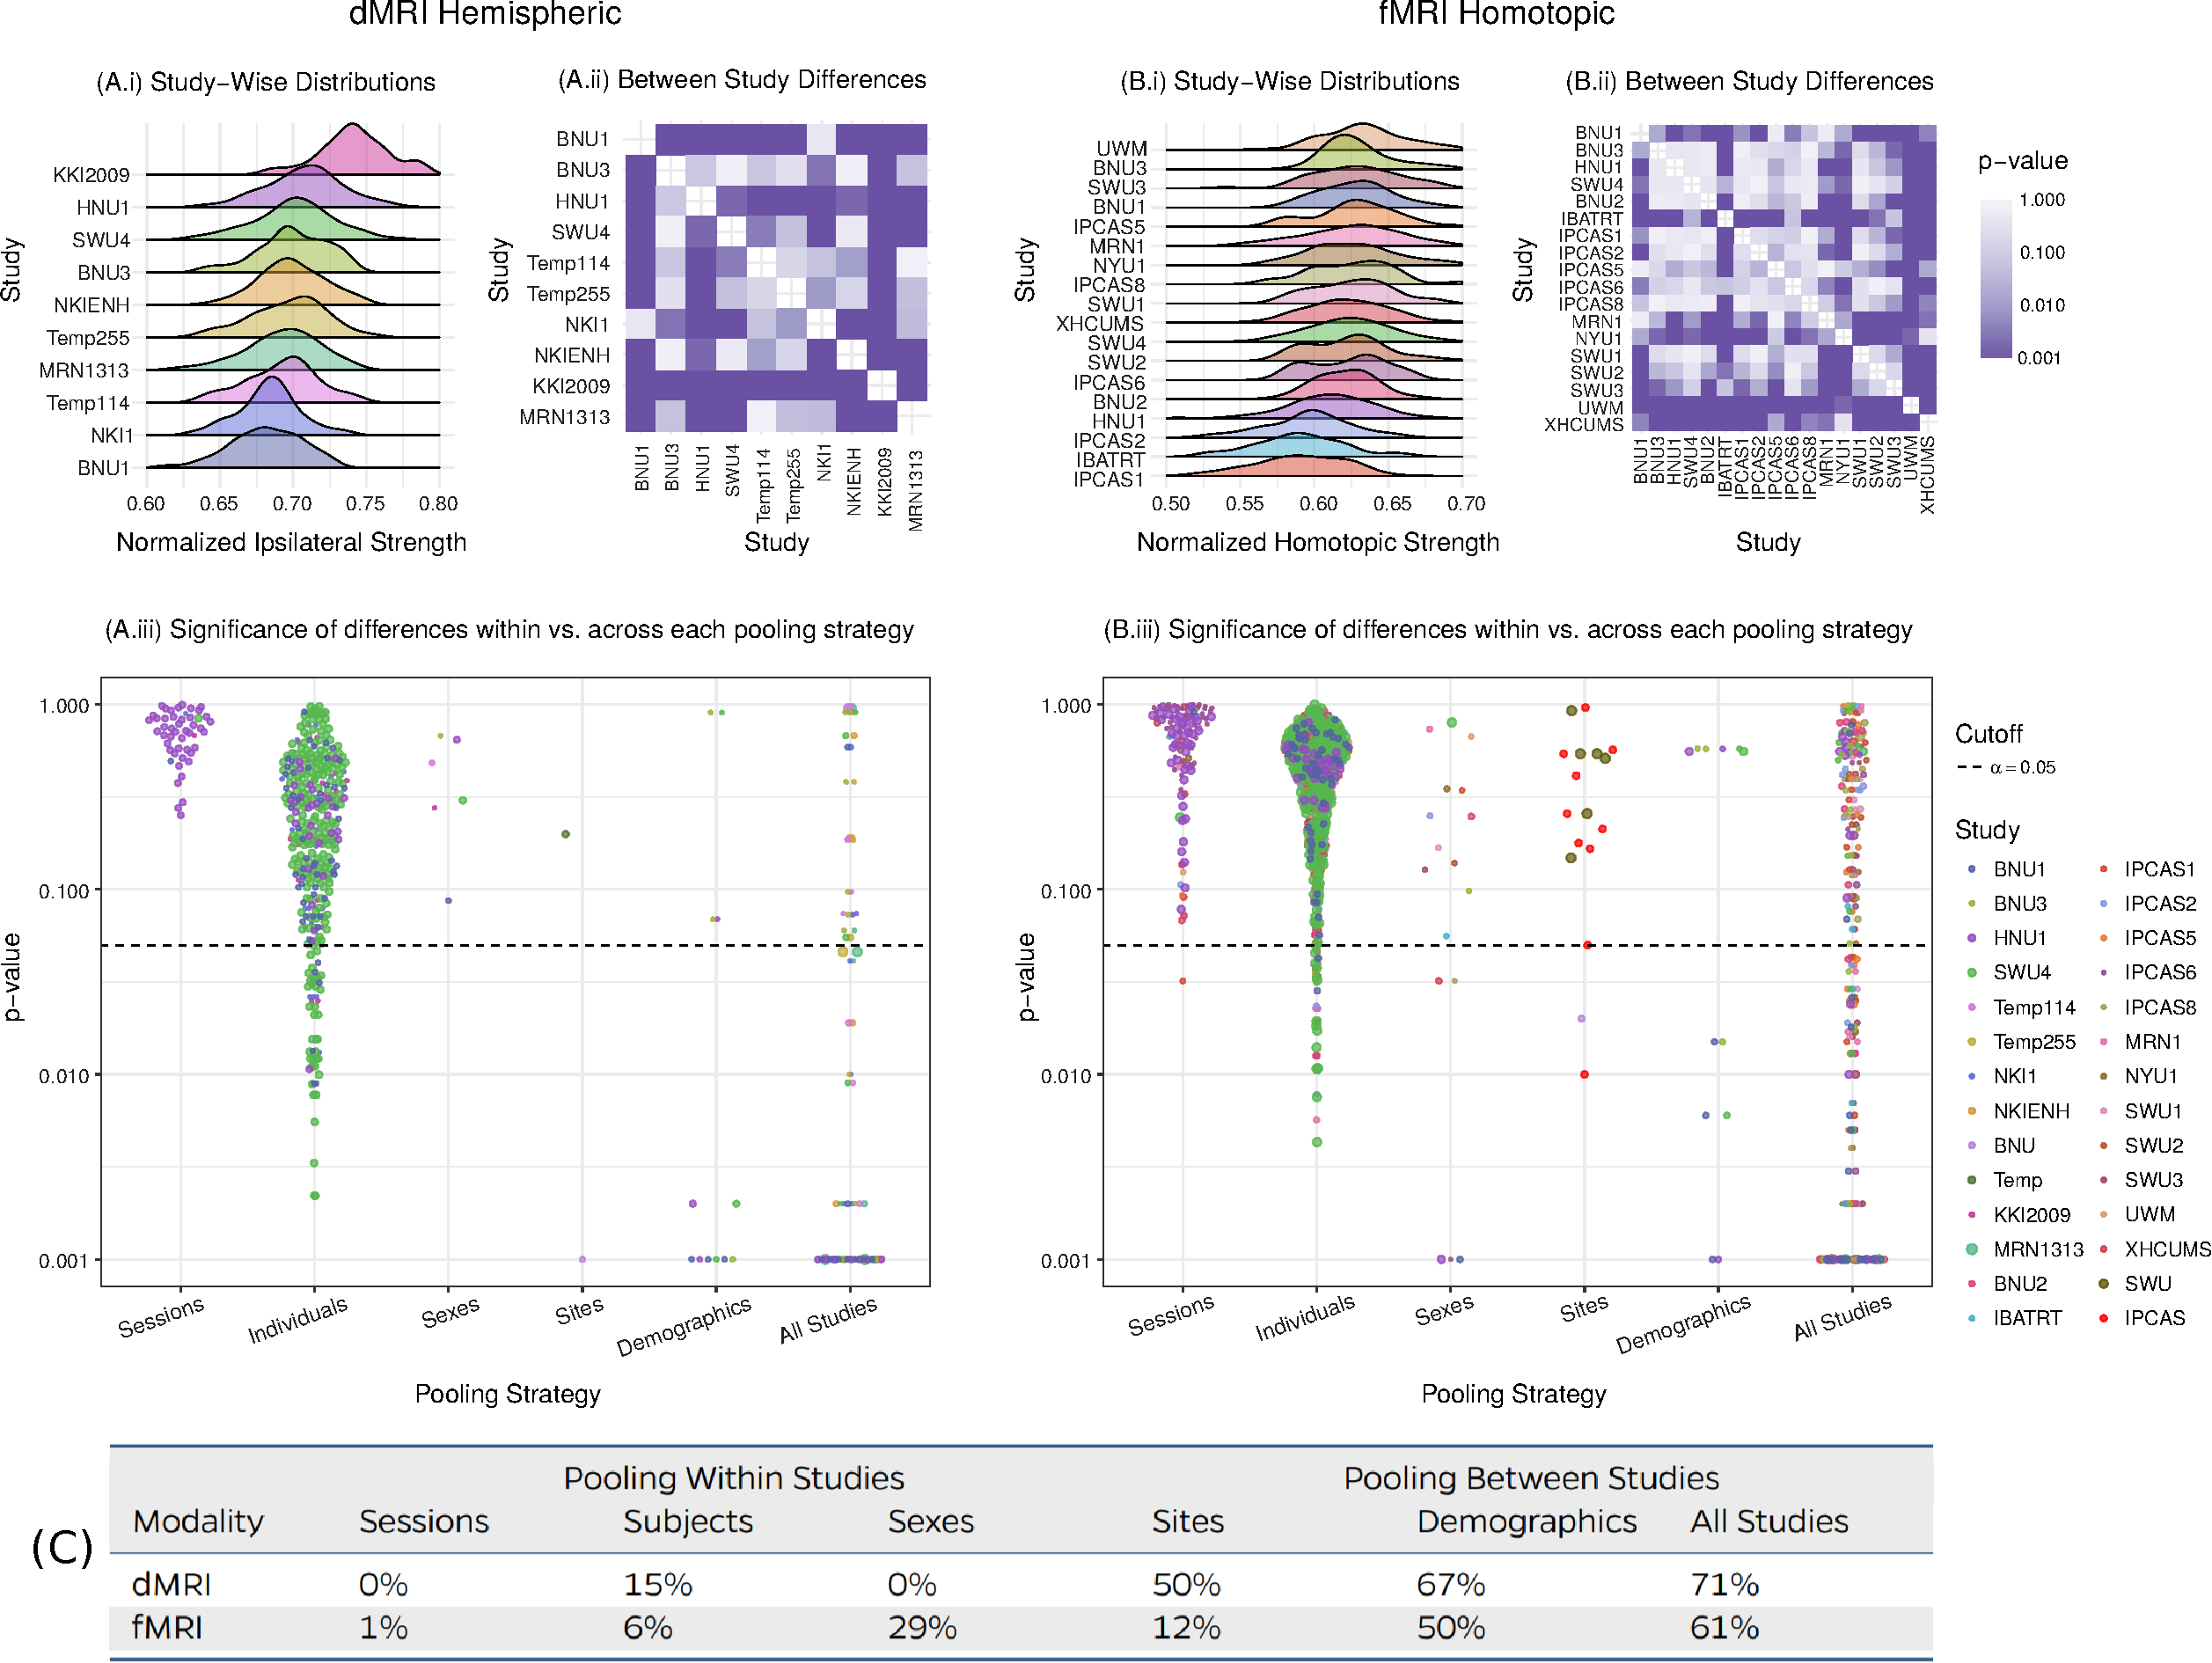
\includegraphics[width=\textwidth]{./figs/fig_batch.pdf}
\end{subfigure}
\caption{\textbf{The prevalence of connectome batch effects are investigated within and across studies using different delineations of the edges into communities for dMRI and fMRI.}
\textbf{(A)} dMRI connectomes delineate edges into within and across hemisphere. 
 \textbf{(B)} fMRI connectomes delineate edges into homotopic and heterotopic edges. 
% batch effects are instead investigated with a homotopic delineation of the vertices, with one community $C_p$ the homotopic edges and the other community $C_q$ the heterotopic vertices. The edge communities were chosen as these communities showed a significant difference in Figure (\ref{fig:siem}), indicating potential for biological signal. 
\textbf{(A.i)} and \textbf{(B.i)} Density estimates of distribution of average ipsilateral or homotopic connection strength within studies. Both within and across study variance is distressingly high.
%the model fit for the ipsi-lateral connections, where $\mathbb{E}\left[\hat{p}\right]$ is the average normalized rank of ipsi-lateral connections or homotopic connections in the dMRI connectomes and fMRI connectomes, respectively. 
\textbf{(A.ii)} and \textbf{(B.ii)} The pairwise significance of  the differences between studies demonstrates that many pairs of studies exhibit significant batch effects. 
%in a paiBatch effect is investigated between each pair of studies. Studies are arranged based on similarity of demographic, where BNU1, BNU3, HNU1, and SWU4 are placed together. $p$-value indicates the significance of a batch effect pooling between the pairs of studies. 
\textbf{(A.iii)} and \textbf{(B.iii)} Several common pooling strategies are investigated, including pooling across  \emph{sessions} within a  study, pooling across \emph{subjects} within a  study, pooling across \emph{sex} within a  study, pooling across studies  from a  scanning \emph{site}, pooling across studies with a similar basic \emph{demographics}, and pooling across \emph{all studies}. In many cases, even when controlling for these factors, significant batch effects remain.
%In each case the number of significant pairs of studies indicates 
\textbf{(C)} The fraction of samples showing significant batch effect at $\alpha = 0.05$. Pooling across sessions, subjects, and sexes,  a small fraction of the samples show significant batch effect in both the dMRI and fMRI connectomes. Pooling across demographics and across all studies  shows  large  batch effects. These results indicate that multiple (typically uncontrolled) variables considerably  impact connectome inferences, implying that  further efforts to mitigate these effects will be required to obtain sufficiently reliable estimates.
}
\label{fig:batch}
\end{figure*}
